\chapter{Detector Response to $^{14}$C Beta Decay}

\section{The Theoretical $^{14}$C Beta-Spectrum}
The shape of the theoretical spectrum of the carbon-14 beta decay has been of interest in the context neutrino mass experiments\cite{C14_Wietfeldt}, where the goal is to measure the precise endpoint, and in liquid scintillator experiments, which have $^{14}$C as a major background and so need to model the spectrum with high precision\cite{C14_Borexino, C14_Bergeron}. This  decay also is of interest in theoretical nuclear physics because it has an abnormally long half life\cite{C14_Kuzminov,C14_Genz,C14_Garcia}. This extended half life hints that there is some cancellation in the lowest order terms of the nuclear matrix element and higher order terms must be taken into consideration. This would also mean that there could be momentum-dependent deviations from the allowed spectral shape. There have been several experiments\cite{C14_Sonntag,C14_Wietfeldt,C14_Borexino,C14_Kuzminov,C14_Bergeron} which have shown deviations from the allowed shape. These results, however, are in some tension with each other, as well as with previous measurements which show a purely allowed spectral shape\cite{C14_Curran}.

\subsection{The Allowed Spectrum}
Carbon-14 decays to the ground state of nitrogen-14 by way of an allowed Gamow-Teller transition. This decay has a Q-value of 156 keV and a half life of 5730 years. In general, the theoretical spectrum for this decay takes the form\cite{C14_Kuzminov}:
\begin{equation}\label{eq:beta_spec}
\frac{dN}{dE}=\frac{1}{2\pi^3} \xi C(E) F(Z,E) p(E_0-E)^2
\end{equation}
Here, $p$ and $E$ are the momentum and total energy of the emitted beta, and $E_0$ is the endpoint energy of the spectrum. In equation \ref{eq:beta_spec} we have neglected the neutrino mass as well as a radiative correction term which is expected to have $<1\%$ effect on the shape of the spectrum\cite{C14_Wietfeldt}. The initial distribution of momentum between the electron and neutrino is proportional to $p(E_0-E)^2$. This is derived by the phase space density of free particles and will be referred to as the phase space factor. The Fermi function $F(Z,E)$ contains information about the interaction between the emitted beta and the daughter nucleus. The terms $\xi$ and  $C(E)$ represent the energy independent and energy independent parts of the nuclear matrix element.

\subsection{The Fermi Function}\label{sec:fermifunc}
As the emitted beta travels away from the daughter nucleus, the two interact and either increase or decrease the momentum of the beta, depending on its charge. In the case of $^{14}C$, the beta has a negative charge and has to climb up out of the electric potential created by the $^{14}N$ daughter nucleus. The resulting observed beta spectrum will then be pulled to lower energy than the initial phase space factor. This modification to the spectrum if known as the Fermi function, $F(Z,E)$. The traditional derivation of $F(Z,E)$ begins by assuming the daughter nucleus is a fixed point charge and then evaluates the electron wave-function given the resulting field. The wave function is only evaluated down to the nuclear radius, $R$, in order to avoid divergence\cite{wilkinson}:
\begin{equation}\label{eq:fermifunc1}
F(Z,E)=2(\gamma+1)\Gamma(2\gamma+1)^{-2}(2pR)^{2(\gamma-1)}e^{\pi \alpha Z E/p}|\Gamma(\gamma+i\alpha ZE/p)^{2}|^2
\end{equation}

There is also a much simpler closed-form solution in the low-Z, non-relativistic approximation\cite{beta_fermi}:
\begin{equation}\label{eq:fermifunc2}
F_{NR}(Z,E)=\frac{x}{1-exp(-x)},
\end{equation}
where $x=2\pi Ze^{2}/\hbar v$. Here, $Z$ is the atomic number of the daughter nucleus, $e$ is the electron charge, and $v$ is the final velocity of the beta particle. 

Electrons in the higher-momentum part of the spectrum will have velocities exceeding 0.5c, so the non-relativistic approximation may not hold. This being the case, we consider the Bethe-Bacher approximation, which estimates the relativistic correction\cite{beta_fermi,bethe}:
\begin{equation}\label{eq:fermifunc3}
F_{BB}(Z,E)=F_{NR}(Z,E)[W^2(1+4\gamma^2)-1]^S,
\end{equation}
where $W\equiv E/m_ec^2$, $\gamma \equiv \alpha Z$, and $S\equiv (1-\gamma^2)^{1/2}-1)$. The full relativistic Fermi function can be estimated by a series expansion on powers of $(\alpha Z)$\cite{wilkinson,C14_Wietfeldt}. This sum is of limited use to us here because it becomes invalid at low kinetic energy and in fact diverges at zero.

The final correction to the Fermi function we consider is the correction for screening of the Coulomb potential by the orbital electrons. This essentially amounts to a shift in the origin of $F(Z,E)$\cite{C14_Wietfeldt,beta_screening}:
\begin{equation}\label{eq:fermifunc4}
F_{S}(Z,E)=\frac{E'p'}{Ep}F(Z,E'),
\end{equation}
where $E'=E-V_0$ and $p'$ is is the associated momentum. For the $^{14}$C beta decay, $V_0=495$eV\cite{C14_Wietfeldt}.

Figure \ref{fig:C14_spec_corrs} compares the non-relativistic approximation to the various corrections described in this section. We can see that the Wilkinson expansion differs from $F_{NR}(7,E)$ by less than a percent down to a few eV, at which point it diverges. The Bethe-Bacher approximation is similarly very close to $F_{NR}(7,E)$, but it does not display the same pathological behavior at the origin. The correction for electron screening peaks at 1.5\% at a kinetic energy of $T=3.5$keV. Because of the pathology in the Wilkinson expansion, we will take our Fermi function to be the combination of equations \ref{eq:fermifunc3} and \ref{eq:fermifunc4}:
\begin{equation}\label{eq:fermifunc5}
F(Z,E)=\frac{E'p'}{Ep}F_{NR}(Z,E')[(E'/m_ec^2)^2(1+4\gamma^2)-1]^S,
\end{equation}
with $F_{NR}(Z,E)$ as defined in equation \ref{eq:fermifunc2} and $E'$ and $p'$ as defined for eqaution \ref{eq:fermifunc4}.

\begin{figure}[h!]
\centering
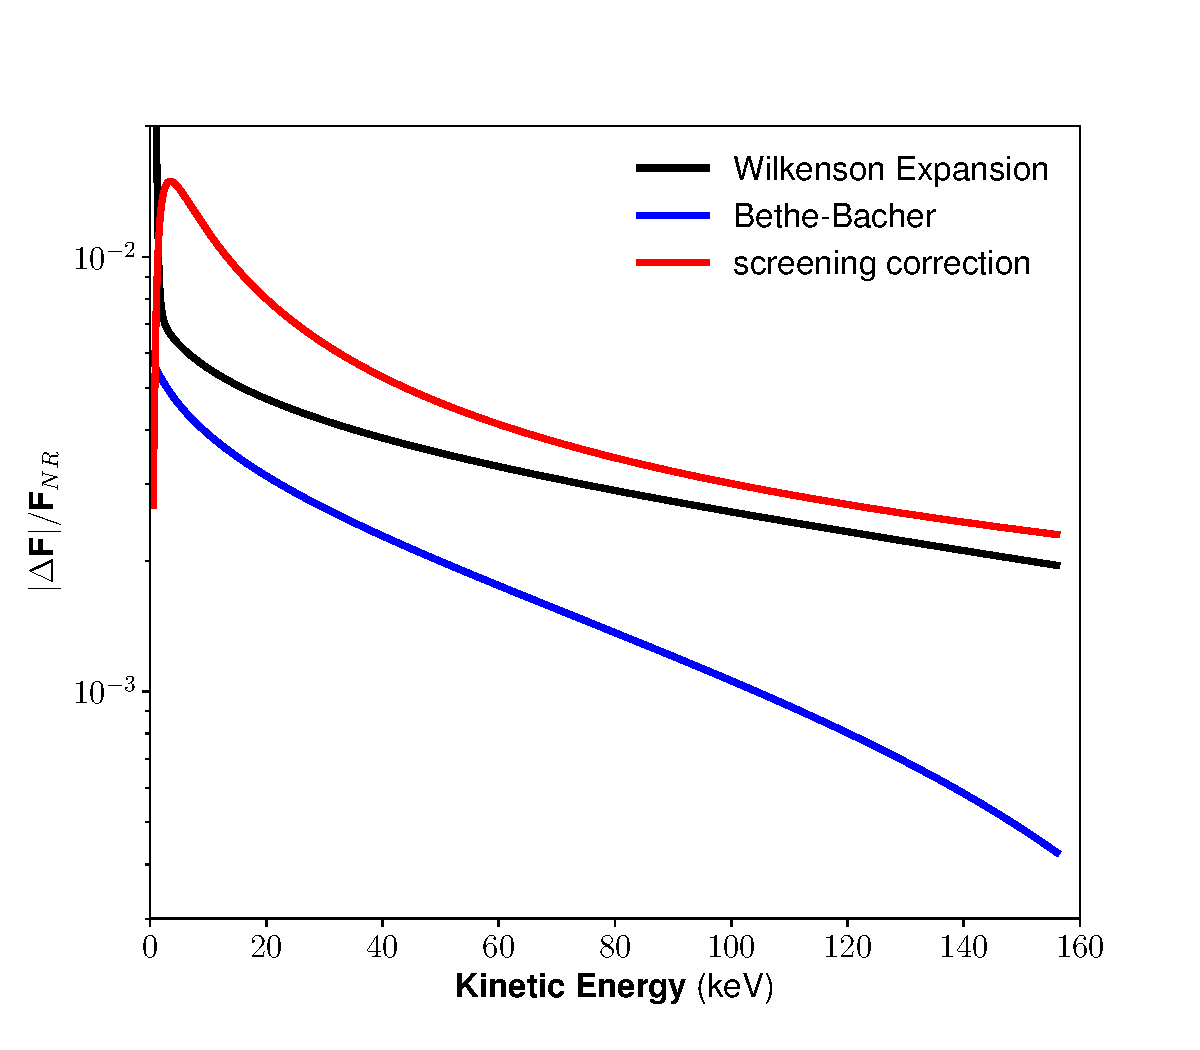
\includegraphics[width=\textwidth]{Figures/FermiFunc_compare.pdf}
\caption{Correction factors for the $^{14}$C beta Fermi function. We compare the non-relativistic approximation, $F_{NR}(7,E)$ to the relativistic corrections described in section \ref{sec:fermifunc}, as well as the non-relativistic function after having been adjusted to account for screening by the orbital electrons. Plotted is $|F'(7,E)-F_{NR}(7,E)|/F_{NR}(7,E)$, where $F'(7,E)$ are the adjusted Fermi functions as indicated in the legend.} 
\label{fig:C14_spec_corrs}
\end{figure}

\subsection{The Shape Factor}
For a typical allowed decay, the shape factor is dominated by interference between the Gammow-Teller axial matrix element, $\langle GT \rangle$ and the weak magnetism matrix element, $\langle WM \rangle$. Such a shape factor has the form\cite{C14_Kuzminov,C14_Garcia,C14_Wietfeldt,beta_Calaprice}:
\begin{equation}\label{eq:shapefactor1}
C(E)\approx1+\frac{4}{3M}\frac{\langle WM \rangle}{\langle GT \rangle}[E-E_0/2-m_e^2/E],
\end{equation}
where $M$ is the nucleon mass, $m_e$ is the electron mass, and $E_0$ is the endpoint energy of the beta-spectrum. Usually the energy dependence of $C(E)$ is small enough that it can be neglected, but in the $^{14}$C beta decay the suppressed decay rate means that $\langle GT \rangle$ is small enough to make its consideration necessary. Under the conserved vector current hypothesis (CVC), the weak magnetism matrix element can be analogized to that of an M1 electromagnetic transition ($\langle WM \rangle$=$\langle M1 \rangle$) for the purpose of calculating the expected shape factor.

There have been several calculations of the predicted shape factor\cite{C14_Garcia,C14_Wietfeldt,C14_Genz}. These typically use a more general form of the $C(E)$ which takes into account terms which have been neglected from equation \ref{eq:shapefactor1}:
\begin{equation}\label{eq:shapefactor2}
C(E)=1+aE+\mu_1\gamma_1b/E+cE^2,
\end{equation}
where $\gamma_1=[1+(\alpha Z)^2]^{1/2}$ and $\mu_1$ is a special Coulomb function. The coefficients $a$, $b$, and $c$ can be calculated using the appropriate matrix elements. The matrix elements are typically calculated using model wave functions for the $^{14}$C and $^{14}$N ground states.

The first measurement of the $^{14}$C shape factor was made by Sonntag et. al. in 1970\cite{C14_Sonntag}. In units of MeV, his measured shape factor was, $C(E)=1-9.14E+1.53/E+7.66E^2$. Genz et. al.\cite{C14_Genz} used this result in part to derive phenomenological wave functions which replicate the shape factor. Later experiments and theoretical calculations have rejected this shape factor.

Wietfeldt et. al. found their data to be consistent with a shape factor of $C(E)=1+aE$, with $a=-0.45 \text{ \ MeV}^{-1}$\cite{C14_Wietfeldt}. This result is very close to their own theoretical calculation of $a=-0.38 \pm 0.04 \text{ \ MeV}^{-1}$, along with theoretical calculations by Garcia and Brown\cite{C14_Garcia}, and  Calaprice and Holstein\cite{beta_Calaprice}. However, the best-fit value of $a$ was inconsistent depending on what range of energies was fit, and a second measurement of the spectrum 2 years later yielded a best fit parameter of $a=-0.63 \pm 0.05 \text{ \ MeV}^{-1}$. 

The Borexino collaboration attempted to measure the shape of the $^{14}$C beta spectrum using their counting test facility (CTF). They assumed the same functional form as the Wietfeldt paper and excluded all $a<-0.72 \text{ \ MeV}^{-1}$ with 90\% confidence\cite{C14_Borexino}. 


Most recently, V. Kuzminov and N. Osetrova measured the shape factor of then $^{14}$C beta decay using a wall-less proportional counter\cite{C14_Kuzminov}. They assumed a shape factor with the form, $C(E)=1+\beta(Q-T)$, with $Q$ being the endpoint energy and $T$ being the kinetic energy of the electron. They measured $\beta=1.24 \pm0.04 \text{ \ MeV}^{-1}$, which is in agreement with a theoretical calculation by . This result is equivalent to $a=0.68 \pm0.02 \text{ \ MeV}^{-1}$ in a Wietfeldt-style shape factor.



\section{Measurement of the Shape of the $^{14}$C Beta-Spectrum}


\section{Measurement of Light and Charge Yields}


\section{Measurement of Recombination Fluctuations from $^{14}$C}